\documentclass[a4paper,11pt]{article}

%%%%%%%%%%%%%%%%%%%%%%%%%%%%%%%%%%%%%%%%%%%%%%%%%%%%%%%%%%%%%%%%%%%%%%%%
% Paquetes utilizados
%%%%%%%%%%%%%%%%%%%%%%%%%%%%%%%%%%%%%%%%%%%%%%%%%%%%%%%%%%%%%%%%%%%%%%%%

% Gráficos complejos
\usepackage{graphicx}
\usepackage{caption}
\usepackage{subcaption}
\usepackage{placeins}

% Soporte para el lenguaje español
\usepackage{textcomp}
\usepackage[utf8]{inputenc}
\usepackage[T1]{fontenc}
\DeclareUnicodeCharacter{B0}{\textdegree}
\usepackage[spanish]{babel}

% Código fuente embebido
\usepackage{listings}

% PDFs embebidos para el apéndice
\usepackage{pdfpages}

% Matemáticos
\usepackage{amssymb,amsmath}

% Tablas complejas
\usepackage{multirow}

% Formato de párrafo
\setlength{\parskip}{1ex plus 0.5ex minus 0.2ex}

% Formato de listados de código
\definecolor{gray}{rgb}{0.5,0.5,0.5}
\lstset{title=\lstname,
  basicstyle=\footnotesize,
  showspaces=false,
  showstringspaces=false,
  breaklines=true,
  commentstyle=\color{gray},
  numbers=left,
  numberstyle=\tiny\color{gray},
  numbersep=5pt,
  frame=single
}

%%%%%%%%%%%%%%%%%%%%%%%%%%%%%%%%%%%%%%%%%%%%%%%%%%%%%%%%%%%%%%%%%%%%%%%%
% Título
%%%%%%%%%%%%%%%%%%%%%%%%%%%%%%%%%%%%%%%%%%%%%%%%%%%%%%%%%%%%%%%%%%%%%%%%

% Título principal del documento.
\title{\textbf{Trabajo Práctico 2: Profiling y optimización}}

% Información sobre los autores.
\author{
  Andrés Gastón Arana, \textit{P. 86.203}                          \\
  \texttt{and2arana@gmail.com}                                     \\
  Sergio Matías Piano, \textit{P. 85.191}                          \\
  \texttt{smpiano@gmail.com}                                       \\ [2.5ex]
  \normalsize{2do. Cuatrimestre de 2012}                           \\
  \normalsize{66.20 Organización de Computadoras}                  \\
  \normalsize{Facultad de Ingeniería, Universidad de Buenos Aires}
}
\date{}

%%%%%%%%%%%%%%%%%%%%%%%%%%%%%%%%%%%%%%%%%%%%%%%%%%%%%%%%%%%%%%%%%%%%%%%%
% Documento
%%%%%%%%%%%%%%%%%%%%%%%%%%%%%%%%%%%%%%%%%%%%%%%%%%%%%%%%%%%%%%%%%%%%%%%%

\begin{document}

% ----------------------------------------------------------------------
% Top matter
% ----------------------------------------------------------------------
\thispagestyle{empty}
\maketitle

\begin{abstract}

  Este informe sumariza el desarrollo del trabajo práctico 2 de la materia
  Organización de Computadoras (66.20) dictada en el segundo cuatrimestre de
  2012 en la Facultad de Ingeniería de la Universidad de Buenos Aires. El mismo
  consiste en la optimización de un sistema de simulación con énfasis en el
  análisis de perfilado y aprovechamiento de cache.

\end{abstract}

\clearpage

% ----------------------------------------------------------------------
% Tabla de contenidos
% ----------------------------------------------------------------------
\tableofcontents
\clearpage


% ----------------------------------------------------------------------
% Desarrollo
% ----------------------------------------------------------------------
\part{Desarrollo}

\section{Algoritmo de implementación}

El sistema analizado simula la evolución de un ecosistema simplificado en un
planeta ficticio toroidal denominado Wator. Para hacerlo, mantiene una matriz
de \(32x32\), donde cada celda representa una unidad de espacio en la
superficie del planeta. La celda está representada por una estructura que
contiene datos acerca del animal que está alojado en ella (tiempo de vida,
hambre y tipo de animal), junto con un flag que marca, para cada iteración, si
la celda ya ha sido procesada o no.

Se inicializa al azar cada una de las celdas, de acuerdo a ciertos parámetros
de distribución de cada tipo de animal, y luego se simulan 1000 turnos de
evolución del ecosistema. En cada turno se procesa secuencialmente cada una de
las celdas de acuerdo al tipo de animal alojado en la celda y las reglas
propias del ecosistema. Al finalizar cada turno se imprime por pantalla o a un
archivo el estado del mapa.

\section{Profiling inicial} \label{sec:profinicial}

Primeramente se examinó el código y se eliminaron algunos problemas en la
estructura del programa. Particularmente se eliminaron las variables sin
utilizar y se unificaron las funciones \textit{choose\_fish} y
\textit{choose\_empty} en una única función: \textit{choose\_random}. Se
decidió hacer esta modificación dado que las funciones eran absolutamente
equivalentes, distinguiendose únicamente por el tipo de celda que buscaban en
el mapa, y unificándolas podemos tener un mejor resultado en el profiling a la
hora de analizar si la estrategia de procesamiento en la búsqueda es la más
adecuada a los parámetros de ejecución del sistema.

Se promedio el tiempo de ejecución del sistema sobre 1000 ejecuciones para
disminuir el error aleatorio en la medición, obteniendo una ejecución
aproximada de 75 milisegundos. Se calculo también el miss rate promedio en el
cache de nivel 1 de las características dadas en el enunciado utilizando
\textit{cachegrind}, siendo este aproximadamente del 30\%.

Se realizó un perfilado de la ejecución del programa utilizando la herramienta
\textit{gprof}. La mayor parte del tiempo de ejecución está concentrado en 3
funciones: \textit{choose\_random}, \textit{move\_to\_fish} y
\textit{move\_to\_empty}. Es en estas tres funciones que nos detendremos
inicialmente para analizar que propuestas de optimización pueden realizarse.

\section{Optimizaciones}

En base a los resultados del perfilado sumarizados en la
sección~\ref{sec:profinicial}, se determinaron diversas alternativas para
intentar mejorar la performance del sistema en la arquitectura detallada en el
enunciado del trabajo práctico. En cada una de ellas se intentó cumplir con uno
de los dos objetivos enunciados a continuación:

\begin{enumerate}

  \item Disminuir la cantidad de accesos a memoria principal y la tasa de falla
      en el cache de la arquitectura propuesta por el ejercicio.

  \item Disminuir la cantidad de operaciones necesarias para alcanzar la
      solución deseada.

\end{enumerate}

Decidimos priorizar el disminuir la tasa de fallas en el cache antes que la
cantidad de operaciones necesarias para calcular la solución. Esta decisión
está basada en el gran impacto que tienen los tiempos de acceso a memoria en el
tiempo de ejecución del programa. Cabe destacar que esta priorización no es
fija, sino que se evalua con criterio: si disminuir el miss rate en un
\(0.01\%\) implica realizar el doble de operaciones, quizás no se observe una
mejora en el tiempo de ejecución sino todo lo contrario. Por otro lado, al
realizar la medición de tiempos de ejecución en una arquitectura con una
estructura jerárquica de memoria completamente diferente a la propuesta por el
trabajo práctico, se espera que disminuir el miss rate no influya directamente,
en esta arquitectura, en el tiempo final de ejecución.

En las siguientes secciones discutimos algunas de las optimizaciones
propuestas, ordenadas de menor a mayor complejidad, incluyendo los motivos que
podrían colaborar a obtener una mejora de performance así como las
consecuencias de su implementación que llevan a empeorar el tiempo de ejecución
del sistema. En cada sección se detallará su implementación y las mediciones
correspondientes a fin de confirmar o rechazar la optimización.

\subsection{Reemplazar variables por constantes}

\subsubsection{Análisis y propuesta}

Existen varias variables a lo largo del código que en realidad son constantes
propagadas. El ejemplo más simple de estas variables fijas son las variables de
parámetros del ecosistema \textit{HBRUT}, \textit{FBRUT} y \textit{FASTEN}. Si
bien están definidas como variables, en realidad se utilizan como constantes
cuyo valor es determinado en tiempo de ejecución en la función \textit{main},
al invocar a la rutina de incialización del mapa.

Se pueden reemplazar estas variables casi sin esfuerzo por constantes. Se
espera que este mecanismo permita al compilador optimizar las instrucciones
ejecutadas para usar algún tipo de acceso a memoria inmediato, eliminando la
necesidad de acceder a memoria para obtener los valores y las complicaciones
adicionales de conflictos en el cache, así como también disminuyendo la
cantidad de operaciones a realizar.

\subsubsection{Implementación}

\lstinputlisting{opt/01constants.diff}

\subsubsection{Resultados obtenidos}

Los resultados fueron bastante buenos para la simplicidad del cambio realizado.
Se obtuvo un tiempo de ejecución promedio de 70 milisegundos, con un speed up
de \(1.07\). Además el miss rate bajó de 30\% a 27\%.

\subsection{Actualizar flag de proceso en una única iteración}

\subsubsection{Análisis y propuesta}

Cada iteración consta de un proceso en el que se actualiza un flag en cada
celda que marca la misma como pendiente. Luego, durante el proceso de cada
celda se marca la misma como procesada a medida que se avanza sobre el mapa.

El objetivo de dicho mecanismo es evitar procesar dos veces el mismo animal.
Como el mapa se recorre desde la celda \((0, 0)\) por fila y columna, puede
darse la situación de que un animal sea procesado y movido hacia posiciones que
no han sido procesadas aún. Este flag evita que se procese dos veces un animal
en estos casos.

Es posible proceder de mantener todas las celdas que ya han sido procesadas y
que no pueden ser reprocesadas como pendientes. El flag se actualiza como
procesado únicamente cuando un animal se mueve a una posición que aún no ha
sido procesada. De esta manera se evita hacer dos pasadas sobre la matriz en
cada iteración, y más importante aún, se evita en muchos casos actualizar un
valor con un write por cada elemento de la matriz.

Por otro lado, dado que el valor del flag es leido inicialmente para evitar
reprocesar, es muy posible que este valor ya esté en la cache al momento de
hacer la escritura, por lo que la ganancia real de performance puede ser muy
acotada.

\subsubsection{Implementación}

\lstinputlisting{opt/02todo.diff}

\subsubsection{Resultados obtenidos}

Como se había previsto, se obtuvo una mejora marginal de performance, con 68
milisegundos de ejecución representando un speed up de \(1.03\). El miss rate,
por otro lado, se mantuvo constante.

\subsection{Recálculo de ubicaciones en interface de \textit{choose\_random}}

\subsubsection{Análisis y propuesta}

La función \textit{choose\_random} computa las nuevas posiciones en i y j para
cada dirección tentativa a elegir. Posteriormente elige una de estas posiciones
al azar y devuelve la dirección correspondiente.

Las funciones que invocan a \textit{choose\_random} toman la dirección devuelta
por esta y recalculan nuevamente las posiciones en i y j para la dirección
elegida.

Es posible devolver una estructura desde la función, equivalente a un word, que
contenga las posiciones calculadas originalmente. De esta manera se evita tener
que recalcular la posición desde las funciones cliente de
\textit{choose\_random}, disminuyendo de esta manera la cantidad de operaciones
necesarias para realizar los cálculos requeridos.

\subsubsection{Implementación}

\lstinputlisting{opt/03recalculo.diff}

\subsubsection{Resultados obtenidos}

Nuevamente se tuvo una mejora marginal, con un tiempo de ejecución de 67
milisegundos y un speed up de \(1.01\), sin cambios en el miss rate.

\subsection{Disminuir el tamaño por celda}

\subsubsection{Análisis y propuesta}

La mayor parte de las fallas en cache se deben al patrón patológico de acceso a
memoria que realiza la función \textit{choose\_random}. Al realizar saltos
entre filas distantes entre si, y teniendo en cuenta que para los parámetros de
cache que se manejan en el ejercicio propuesto entran muy pocas celdas por
linea de cache, exiten muchas fallas de cache por conflicto entre lineas
reemplazadas.

Una posible optimización, dedicada exclusivamente a mejorar algo la tasa de
fallas de cache, es disminuir el tamaño de la estructura de datos almacenada en
cada celda de la matriz, de manera de aumentar la cantidad de celdas que entran
en cada linea de cache. Es posible disminuir a la mitad el tamaño eligiendo los
tipos de datos adecuados.

\subsubsection{Implementación}

\lstinputlisting{opt/04tam.diff}

\subsubsection{Resultados obtenidos}

Si bien se obtuvo un tiempo de ejecución ligeramente mayor (con 68 milisegundos
contra 67 milisegundos antes de esta optimización), se obtuvo una mejora
sustancial en el miss rate, bajando a 22\% desde 27\%. Consideramos que una
mejora de 5\% en el miss rate como la que experimentamos implicaría, en la
arquitectura propuesta por el enunciado, una disminución en el tiempo de
ejecución que superaría ampliamente el costo pagado.

\subsection{Separación de datos por estrategia de acceso a memoria}

\subsubsection{Análisis y propuesta}

Existen dos estrategias de acceso a memoria diferentes al mapa de animales según el tipo de información que se quiera extraer del mismo:

\begin{description}

    \item[Tipo de animal] El tipo de animal alojado en una celda se utiliza
        principalmente en la función \textit{choose\_random}. Esta función
        tiene una estrategia de acceso a memoria patológica, en donde se buscan
        las celdas contiguas en la matriz para cada celda. Esto implica accesos
        consecutivos a filas diferentes y distantes en memoria.

    \item[Parámetros del animal] Los parámetros del animal se utilizan en la
        decisión del comportamiento del mismo de acuerdo a las reglas definidas
        para la evolución del ecosistema. El acceso a memoria para estos datos
        es primordialmente secuencial, a diferencia del caso anterior, y
        aprovecha algo mejor la estructura contigua de los datos en las lineas
        de cache.

\end{description}

En función de este análisis, se detecta la posibilidad de separar estos datos
en dos estructuras paralelas. La primera consiste en una estructura muy
compacta con la información del tipo de animal alojado en cada celda
únicamente. Por el patrón de acceso a esta información, el objetivo es que en
cada linea de cache entre la mayor cantidad posible de este tipo de dato.

Por otro lado, la información sobre los parámetros del animal, al ser accedida
secuencialmente, puede mantenerse en una estructura similar a la
utilizada actualmente.

Si bien esto aumenta la complejidad (particularmente, la actualización de dos
estructuras de datos en vez de una y el mapeo de direcciones entre una y otra)
y con esto la cantidad de operaciones a ejecutar, se espera una mejora
apreciable en la tasa de fallas en cache.

Esta optimización fue analizada teoricamente, sin embargo llevarla a la
práctica implicó gran cantidad de cambios sobre los que ya hemos presentado.
Debido a la manutención de dos estructuras actualizadas al mismo tiempo. La
falta de tiempo para terminar de completarla nos llevó a dejarla como una
alternativa teórica.


\section{Conclusiones}


\clearpage

\part{Apéndice}
\appendix

\section{Enunciado original}\label{sec:enunciado}
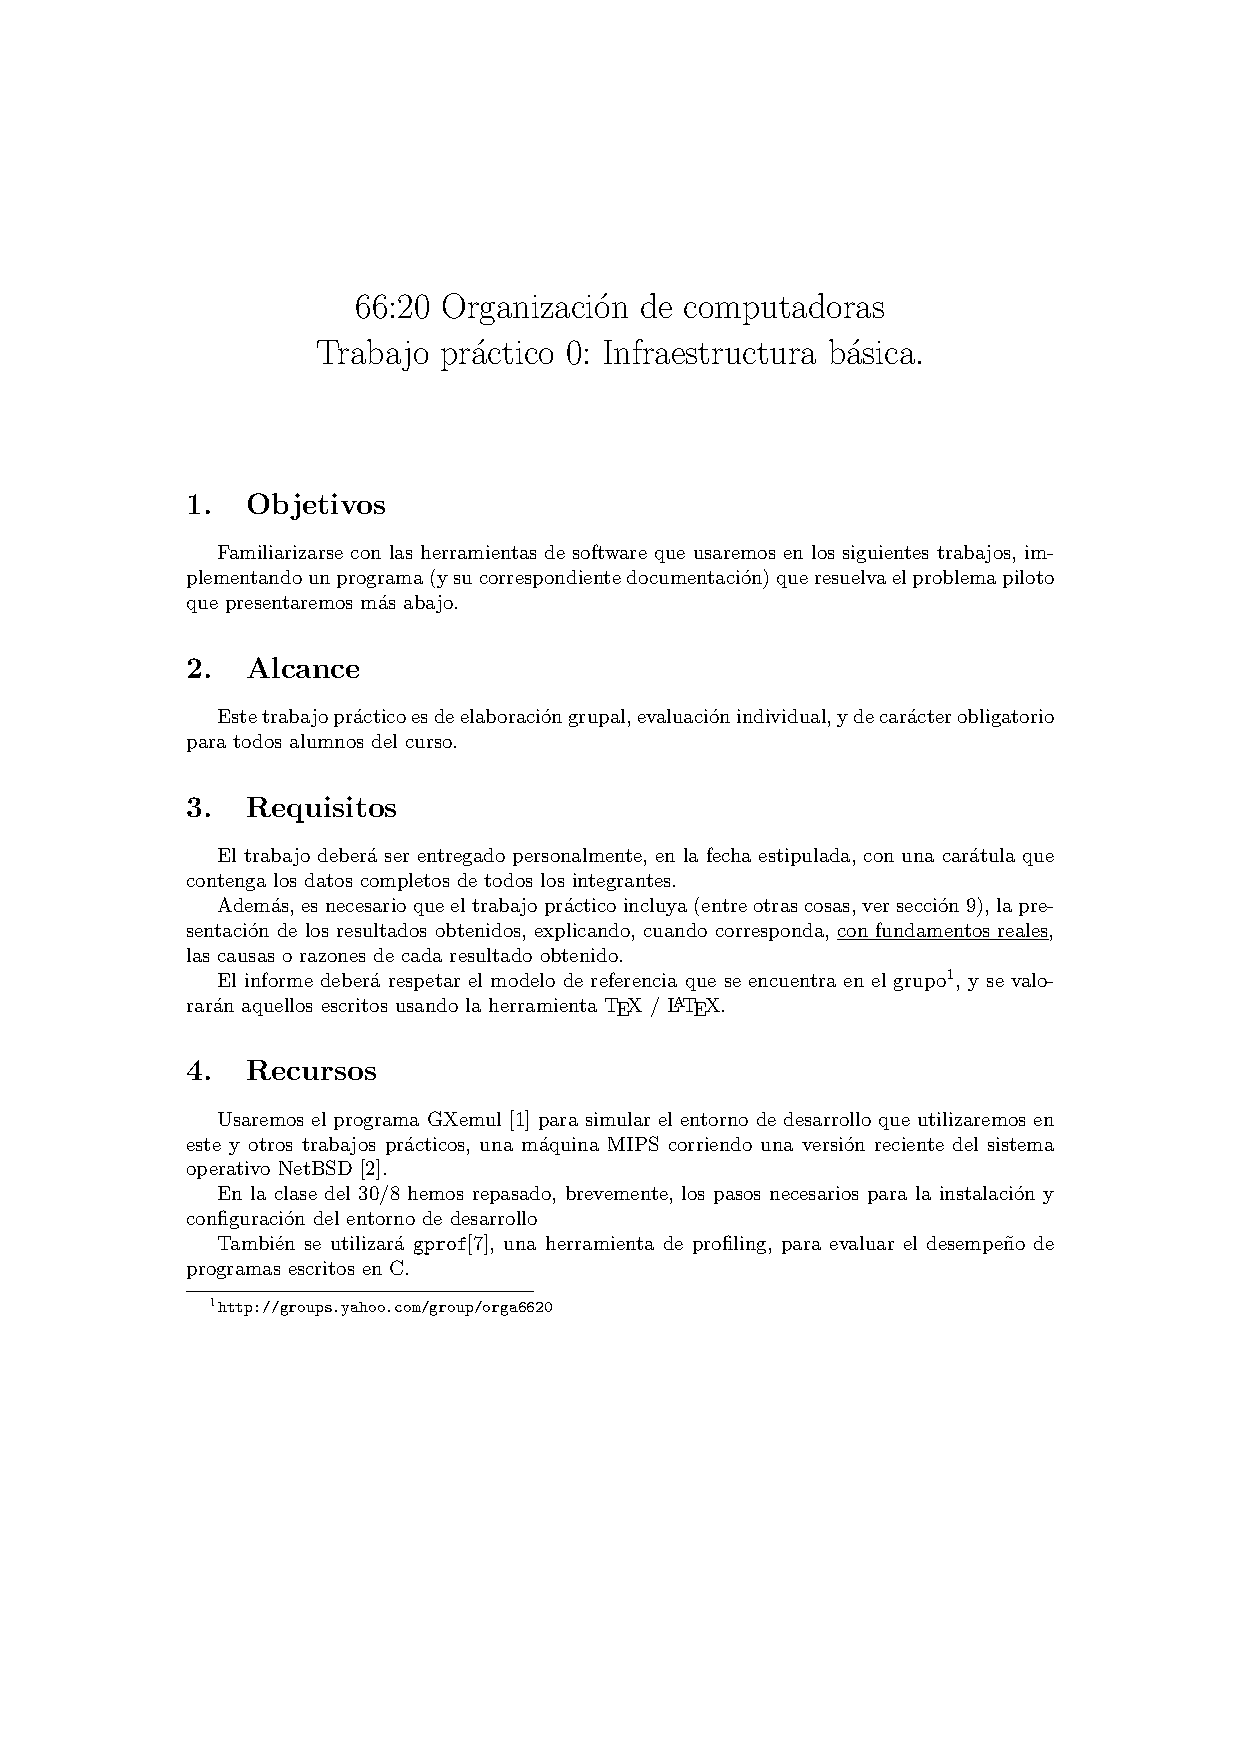
\includepdf[pages={-}]{docs/enunciado.pdf}

\clearpage
\section{README del material digital}\label{sec:readme}
\includepdf[pages={-}]{build/doc/README.pdf}

\clearpage
\section{Código fuente optimizado}\label{sec:source}
\clearpage
\lstinputlisting{source/wator.c}

\end{document}

